\documentclass[10pt]{report}
\usepackage[a4paper]{geometry}
\usepackage[myheadings]{fullpage}
\usepackage{fancyhdr}
\usepackage{lastpage}
\usepackage{graphicx, wrapfig, subcaption, setspace, booktabs}
\usepackage[T1]{fontenc}
\usepackage[font=small, labelfont=bf]{caption}
\usepackage{fourier}
\usepackage[protrusion=true, expansion=true]{microtype}
\usepackage[english]{babel}
\usepackage{sectsty}
\usepackage{url, lipsum}
\usepackage{comment}
\graphicspath{ {images/} }

% Setup in line code
% copied from https://tex.stackexchange.com/questions/19004/how-to-format-an-inline-source-code
\usepackage{listings}
\usepackage{color}
\definecolor{lightgray}{gray}{0.9}
\definecolor{dkgreen}{rgb}{0,0.6,0}
\definecolor{mauve}{rgb}{0.58,0,0.82}
\lstset{
    showstringspaces=false,
    basicstyle=\ttfamily,
    keywordstyle=\color{blue},
    commentstyle=\color[grey]{0.6}
    stringstyle=\color[RGB]{255,150,75}
}

\newcommand{\inlinecode}[2]{\colorbox{lightgray}{\lstinline[language=#1]$#2$}}


\newcommand{\HRule}[1]{\rule{\linewidth}{#1}}
\onehalfspacing
\setcounter{tocdepth}{5}
\setcounter{secnumdepth}{5}

% HEADER & FOOTER
\pagestyle{fancy}
\fancyhf{}
\setlength\headheight{15pt}
\fancyhead[L]{Student ID: 1000921236}
\fancyhead[R]{University of Texas at Arlington}
\fancyfoot[R]{Page \thepage\ of \pageref{LastPage}}


% TITLE PAGE
\begin{document}

\title{ \normalsize \textsc{IE 3301 - 004 Honors\\ Engineering Probability}
        \\ [2.0cm]
        \HRule{0.5pt} \\
        \LARGE \textbf{\uppercase{Analysis of UTA Student Feedback Survey Results}} \\
        \normalsize \textit{using Simple Linear Regression}
        \HRule{2pt} \\ [0.5cm]
        \normalsize \today \vspace*{5\baselineskip}}

\date{}

\author{
    Joe Cloud \\
        Student ID: 1000921236 \\
        University of Texas at Arlington \\[1in]
        \textit{I, Joe Cloud, did not give or receive any assistance on }\\
        \textit{this project, and the report submitted is wholly my own.}}



    \maketitle
\tableofcontents
\newpage

%-------------------------------------------------------------------------------
% Section title formatting
\sectionfont{\scshape}
%-------------------------------------------------------------------------------

% BODY
\section*{Introduction}
\addcontentsline{toc}{section}{Introduction}
Near the conclusion of each semester at UT Arlington (UTA), students are asked to submit their unbiased, anonymous comments
and ratings on the instructors of each of the classes they took. According to the Student Feedback Survey (SFS) website, 
the surveys are designed to "[give] students an opportunity to reflect upon their experience in each organized course", and
to "help members of the faculty identify which aspects of a course should remain unchanged and which aspects might benefit
from revision". \\ 
Once the survey deadline passes, the data is compiled and shared to the academic departments and is made available online
for all students to access (www.uta.edu/ier/Surveys/SFS/the-results.php). It is one of many resources used by students to help them decide which
courses to take in following semesters.  \\
The public data contains various performance metrics such as how well a student felt an instructor encouraged
him/her to take an active role in his/her learning, or how accessible an instructor was in person or electronically, etc. \\
Simple Linear Regression (SLR) is a useful tool for making predictions with continuous data and modeling relationships between
a dependent variable and one (or more, if Multiple Linear Regression) independent variable.
In this report, I explore modeling a relationship between the independent variable "How clearly were the course objectives defined"
and the selected dependent variable "how well an instructor was prepared for instructional activity". I found that there is
indeed a relationship between the two variables, and discussed reasons why this would not be a surprising conclusion.

\newpage

\section*{Data}
\addcontentsline{toc}{section}{Data}
The original publically available dataset is contained in a PDF file. In it there are six columns, the first being the 
name of the instructor and the course number, and the remaining five being the performance metrics that students were asked
to score. For performing SLR only two columns from the data were necessary. As mentioned previously in the Introduction,
I chose to work with the column values for how clearly students felt objectives were defined for the course, and how 
well students felt instructors were prepared for each lecture/lab. \\ 

Each row contained a specific course section and instructor. The values for the performance metrics for each course section
contained mean value students responses since each section was made up of one or more students. The standard deviations 
and number of students enrolled were also provided. In all, over 23,000 data samples were collected; of which I used 696.
My 696 datapairs (X, y) were further divided into two parts, 2/3 for training the line fitter and 1/3 for testing. This 
split of the data was preceeded by shuffling of the data, to prevent repeat instructors from causing overfitting 
during training. 

\begin{wrapfigure}[14]{r}{0.50\textwidth}
    \centering
    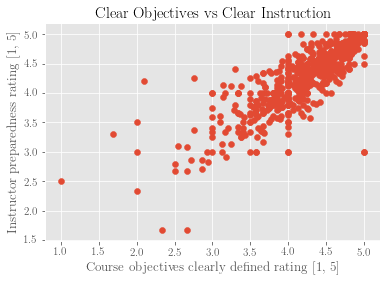
\includegraphics[width=0.50\textwidth]{results/first_plot}
    \caption{Training data}
\end{wrapfigure}

\vspace{5mm}

I am interesting in analyzing these sets because I suspect that an instructor who does not develop (or rather, students who 
don't sense) a clear plan for how a course will be taught are more likely to be ill-prepared for presenting 
content to students throughout the semester. Now of course, there are many other reasons that this data may be correlated. \\ 
Perhaps a student wasn't or was very fond of the instructor regardless of their teaching ability, this could 'skew' results
in the data since the responder may opt to vote all high or low without serious consideration. 
For this reason, data with low standard deviations were favored since it showed greater consensus amongst all
students in a course section. With that being said, results with a standard deviation of 0 are not desired as this would cause the 
results to be integer values (since students are only able to select discrete integer values). \\

In order to collect the data for analysis, the PDF was downloaded from the UTA SFS page and then piped through a PDF to CSV
converter to extract the raw text.This helped make the data accessible for parsing. I then wrote a script (APPENDIX) that would strip out
lines of interest and combine them into a file that could later be used to extract each individual column. This was done
by using the spacing between each column as a delimiter for the values, since the columns are unevenly spaced throughout
the CSV file. Once columns of interests were extracted, they were stored into separate files that could then be loaded into
a python script to perform SLR and accompanying analysis.

% Data analysis
\newpage
\section*{Linear Regression}
\addcontentsline{toc}{section}{Linear Regression}

The heart of this report is the use of SLR to find a line that models the relationship between our two variables in question. 
These variables are referred to by many different terms- for the sake of consistency I will refer to them as the independent and
dependent variables.  With SLR, we are modeling the relationship through a simple linear equation, typically written as
$ \hat Y = b_0 + b_1x$ where $\hat Y$ estimates the true linear equation $\beta_0 + \beta_1x$. \\
SLR was performed using the scikit-learn package, with python. In figure 1 it was fairly easy to spot a trend in the data that indicates
a positive relationship between variables. And the regression line as expected finds its way along that path, shown in figure 2.


\begin{wrapfigure}[14]{r}{0.50\textwidth}
    \centering
    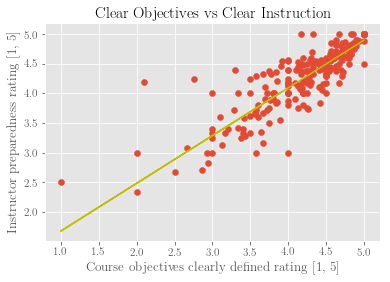
\includegraphics[width=0.50\textwidth]{results/third_w_slr}
    \caption{Testing data with regression line}
\end{wrapfigure}


It is clear from the line that there is a strong positive linear relationship between the data. This also gives us the values
for the $\beta_*$ parameters, with our estimated $\hat Y = 0.8048x + 0.8740$, note that this value will vary depending on how the data
is shuffled, as each time the analysis is performed a different set of training and testing set is produced using
the same 696 sample pairs. In order to perform a thorough analysis, it is also important to consider some other performance metrics.
One indicator is the R-squared value. The R-squared value is a percentage measure indicating how close the data points are with regard
to the regression line. A high R-squared value is preferred, and generally a value above 0.50 or 50\% is considered good. 
In the case of this dataset, we obtained an R-squared value of 70.64\%, a very good value. 

\begin{wrapfigure}[14]{l}{0.50\textwidth}
    \centering
    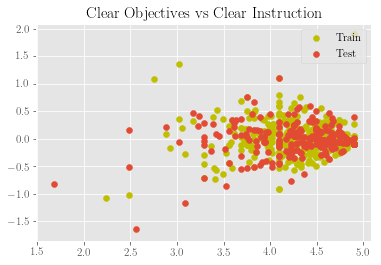
\includegraphics[width=0.50\textwidth]{results/residual}
    \caption{Residual plot}
\end{wrapfigure}

Although a high R-squared value is generally a great result, it is not an adequate condition for stating a regression model is reliable. 
We should also consider the residual plots to get a more comprehensive view. The residual plot is a measurement of the predicted
values subtracted from the observed. Ideally we would see random clustering around 0 on the x-axis, as this would indicate that there 
isn't an inbalance where the regression prediction being much greater, or smaller than the actual values. In addition to this, it helps
to take into accounts some other error metrics, and then take the mean of the errors. One such value is the Mean Squared Error, 
which simply measures the the difference between the predicted values with raw points. This is used to calculate the R-squared value
discussed above. \\
It is worth noting that although regression is a powerful tool for predicting outcomes based on previous data, in this case it was useful
strictly for predicting values based on test data, so then the error could be assessed. This error measurement is important to better
understand how 'reliably' the line performs. 





\newpage
\section*{Conclusion}
\addcontentsline{toc}{section}{Conclusion}

In conclusion, the performance from regression shows a strong correlation between our two variables. Using the analysis we cannot conclude
the reasoning for the relationship. But with careful data processing and selection, as well as some understanding of the motives of survey 
submitters- it is plausible to think that students would score an instructor's preparedness differently given that course objectives are
clearly defined. Considering the slope of the regression line is not $1$ it also makes sense to disregard the idea that students are choosing
to score with extremes based on their overall bias for or against an instructor, this is in part due, again to selection of data with relatively
low standard deviations. The errors measured and residuals also help indicate that the regression line is able to predict with 70\% accuracy the 
result of instructor preparedness given how clearly they define objectives at the beginning of a semester. \\




\newpage
\section*{Appendix}
\addcontentsline{toc}{section}{Appendix}

\begin{table}
    \centering

	\begin{tabular}{rrrrrrrrrrrr}
	\hline
	4.545 & 4.273 & 3.333 & 4     & 3.333 & 3.333 & 4     & 5     & 4     & 3.333 & 5     & 5     \\
	4.231 & 4.19  & 4.154 & 4.19  & 4.083 & 4.5   & 3.846 & 4     & 3     & 3.125 & 3     & 4.556 \\
	4.5   & 2.667 & 4.455 & 4.6   & 4.75  & 4.455 & 3.556 & 4.5   & 4.563 & 3.875 & 3.5   & 4.353 \\
	5     & 4.313 & 4.286 & 4.333 & 4.833 & 4.917 & 2.545 & 2.75  & 3.846 & 4     & 4.571 & 3.9   \\
	4     & 4.75  & 4.25  & 4.4   & 4     & 4.286 & 3.583 & 3.5   & 4.733 & 4.813 & 4.429 & 4.25  \\
	4.474 & 5     & 5     & 4     & 4.4   & 4.5   & 4.067 & 4.25  & 4.481 & 4.75  & 4.556 & 4.455 \\
	3.167 & 4.111 & 3.867 & 3.733 & 4.5   & 4.8   & 4.5   & 4.833 & 4.5   & 4.4   & 5     & 4.625 \\
	4.75  & 4.5   & 4.571 & 4.375 & 4.833 & 4.875 & 4.545 & 4.857 & 4.25  & 4.875 & 4.733 & 4.571 \\
	5     & 4.667 & 4.4   & 3.889 & 3.1   & 4.273 & 4.222 & 4.286 & 4.25  & 4.5   & 4.5   & 5     \\
	4.167 & 4     & 3.5   & 4.333 & 4.083 & 5     & 4.167 & 4.583 & 4.133 & 4.167 & 4     & 4.667 \\
	5     & 4.25  & 4     & 4.25  & 4.167 & 4.5   & 4.75  & 5     & 4.8   & 3.875 & 4.6   & 4.818 \\
	5     & 4.769 & 4.273 & 5     & 4.833 & 5     & 4.6   & 3.571 & 3.545 & 4     & 4.474 & 4.05  \\
	4.25  & 4.143 & 4.182 & 4     & 3.909 & 4.167 & 4     & 3.857 & 4     & 4.333 & 4     & 4.1   \\
	4.143 & 4.333 & 4     & 5     & 3.923 & 4.176 & 4.7   & 4.538 & 3.75  & 4.286 & 5     & 3.857 \\
	2.714 & 4.429 & 4.636 & 2     & 4.25  & 3.9   & 3.6   & 4.833 & 4.25  & 4.636 & 4.556 & 4.923 \\
	4.8   & 4.737 & 4.588 & 4.222 & 4.2   & 4.308 & 4.25  & 2.667 & 4.643 & 4.429 & 5     & 4.568 \\
	4.417 & 4.3   & 3.864 & 3.917 & 5     & 4.571 & 4.6   & 3.556 & 4.133 & 4.286 & 4     & 4.235 \\
	3.909 & 4.368 & 4.667 & 4.545 & 4.556 & 5     & 3.857 & 4.227 & 4.2   & 4     & 4.267 & 4     \\
	4.483 & 4.455 & 4.625 & 4.222 & 4.636 & 4.778 & 4.6   & 4.846 & 5     & 4.778 & 5     & 3     \\
	4.667 & 4.3   & 5     & 4     & 4.667 & 4.769 & 4.5   & 4.571 & 4.667 & 4.3   & 5     & 4.667 \\
	4.286 & 3.538 & 4.75  & 4.556 & 3.25  & 4.231 & 4.818 & 3.667 & 4.333 & 4.857 & 4.111 & 4.267 \\
	4.4   & 4.538 & 4.333 & 4.4   & 4.2   & 4.944 & 4.65  & 4.8   & 4.4   & 4.571 & 4.4   & 4.667 \\
	4.286 & 4.8   & 4.667 & 4.25  & 3.625 & 4.444 & 3.923 & 3.5   & 4.022 & 3.375 & 4.222 & 4     \\
	4.5   & 4.5   & 2.857 & 3.571 & 3.571 & 3.636 & 4.375 & 4.429 & 4.111 & 4.6   & 3.25  & 4.222 \\
	4.182 & 3.778 & 4.125 & 4.5   & 4.429 & 3.333 & 4.75  & 4.579 & 4.182 & 4.069 & 5     & 4.059 \\
	4.563 & 4.8   & 4.667 & 3.857 & 3.667 & 4.25  & 4.364 & 4.571 & 4.667 & 4.167 & 4     & 3.667 \\
	4.111 & 4.4   & 4.875 & 4.917 & 4.667 & 4.444 & 3.667 & 3.583 & 3.867 & 3.655 & 3.852 & 4.125 \\
	3.7   & 4.2   & 3.5   & 3.133 & 3.8   & 2.5   & 2.333 & 4.333 & 4.6   & 4.25  & 4.2   & 4.429 \\
	4.5   & 4.444 & 4.5   & 5     & 4     & 4.5   & 3.667 & 4.875 & 4.091 & 4.182 & 4.385 & 4.182 \\
	4.7   & 4.714 & 4.8   & 3.143 & 5     & 4.833 & 4.667 & 5     & 4.714 & 4.8   & 4     & 3.6   \\
	5     & 4.429 & 4.143 & 5     & 3.75  & 3.8   & 4     & 4     & 3.8   & 5     & 4.714 & 4.667 \\
	4.5   & 5     & 4.25  & 4.148 & 4.222 & 4.2   & 1.692 & 3.8   & 4.875 & 3.375 & 4     & 3.8   \\
	3.3   & 4.2   & 3.889 & 4.385 & 4.875 & 4.417 & 4.333 & 4.143 & 4     & 3.667 & 3.833 & 5     \\
	4.417 & 4.6   & 4.889 & 4.5   & 4.571 & 4.667 & 4.429 & 4.778 & 5     & 4     & 4.6   & 3.833 \\
	4     & 4     & 4.333 & 3.4   & 4.875 & 4.333 & 4.857 & 4.667 & 4.125 & 4.111 & 4.318 & 4.714 \\
	4.161 & 4.417 & 3.913 & 3.684 & 3.905 & 4.526 & 4.2   & 4.778 & 3.909 & 3.5   & 4.696 & 4     \\
	4.25  & 4.467 & 3.182 & 3.556 & 5     & 4.889 & 4.222 & 4.4   & 4.5   & 3.857 & 4.211 & 4.476 \\
	4.143 & 3.667 & 4.7   & 5     & 5     & 4.917 & 4.846 & 4.909 & 5     & 3.364 & 4.333 & 3.857 \\
	4.125 & 4.2   & 4.059 & 3.938 & 4.067 & 4.875 & 5     & 4.4   & 4.545 & 4.25  & 5     & 4.273 \\
	4.667 & 4.571 & 4.909 & 4.5   & 4.538 & 5     & 4.125 & 4.3   & 4.6   & 4.857 & 4.5   & 3.714 \\
	4.25  & 3.571 & 4.5   & 4.214 & 4.667 & 4.8   & 4.167 & 4     & 3.3   & 4.2   & 4.421 & 4.5   \\
	4.091 & 3.333 & 4     & 2.941 & 4.75  & 3.6   & 4     & 4.5   & 4.516 & 4.714 & 4.556 & 3.833 \\
	4.429 & 4.667 & 3.818 & 4.75  & 4.667 & 5     & 5     & 4.5   & 2.857 & 3.167 & 4.2   & 4.267 \\
	4.286 & 3.1   & 2     & 4.167 & 4.857 & 4.5   & 4.25  & 3.5   & 4     & 3.571 & 4.125 & 4.2   \\
	4.571 & 4.556 & 4.667 & 4.786 & 4.667 & 4.625 & 4.125 & 5     & 3.2   & 3.5   & 3     & 4.2   \\
	4.308 & 3     & 5     & 4.571 & 4     & 4     & 4.714 & 4     & 4     & 4.5   & 4.2   & 4.5   \\
	4.4   & 4.625 & 4.8   & 4.7   & 4.25  & 4.636 & 5     & 4.5   & 4.5   & 5     & 4.833 & 4.5   \\
	5     & 3.909 & 4.167 & 4.462 & 4.448 & 4     & 3.5   & 2.75  & 4.727 & 4.8   & 3.889 & 4.714 \\
	4.1   & 4.818 & 4.429 & 4.571 & 4.615 & 4.636 & 4.133 & 4.333 & 4.571 & 4.786 & 4.941 & 4.833 \\
	4.3   & 3     & 4.8   & 4.25  & 4.667 & 4.818 & 4.556 & 3.559 & 3.409 & 5     & 5     & 4     \\
	4.7   & 4.667 & 4.75  & 4     & 3.417 & 3.7   & 3.375 & 3     & 3.333 & 3.6   & 3     & 2.5   \\
	4.091 & 4.727 & 4.714 & 4.571 & 4.6   & 4.625 & 3.75  & 2.1   & 3.75  & 2.923 & 3.75  & 4.421 \\
	4.19  & 3.833 & 4.833 & 4.667 & 4.667 & 3.8   & 3.857 & 4.7   & 4.25  & 4.727 & 4.8   & 4.286 \\
	4.333 & 4.25  & 4     & 3.765 & 4.667 & 4.625 & 4.875 & 5     & 4.167 & 5     & 4.429 & 3.714 \\
	3.125 & 4.143 & 4.333 & 5     & 4.9   & 3.556 & 4.5   & 3.286 & 3.857 & 4.231 & 3.429 & 2.667 \\
	3.5   & 4.182 & 4.4   & 1     & 4.2   & 2     & 3.667 & 4     & 4.2   & 3.4   & 4.462 & 3.8   \\
	3.643 & 4.25  & 4.333 & 3.571 & 4     & 4.75  & 3.667 & 4.4   & 5     & 4.364 & 4     & 4.3   \\
	4.562 & 4     & 4.9   & 3.818 & 3.7   & 4.154 & 3.8   & 4.444 & 3.667 & 4.5   & 3.778 & 3.917 \\
	\hline
	\end{tabular}

    \caption{Independent variable: How clearly were objectives defined [1, 5]}
\end{table}


\begin{table}
    \centering
	\begin{tabular}{rrrrrrrrrrrr}
	
	\hline
	4.818 & 4.273 & 3.667 & 4.188 & 4     & 4     & 4.2   & 5     & 3     & 3.333 & 5     & 5     \\
	4.077 & 4.19  & 4.231 & 4.095 & 4.25  & 4.5   & 3.923 & 3.789 & 3.583 & 3     & 3.75  & 4.444 \\
	4.833 & 1.667 & 4.545 & 4.7   & 4.636 & 4.182 & 3.667 & 4.5   & 4.625 & 4.375 & 3     & 4.353 \\
	4.9   & 4.406 & 4.571 & 3.833 & 4.833 & 4.75  & 3.091 & 3.375 & 4.077 & 4     & 4.571 & 3.6   \\
	3.933 & 4.778 & 4.125 & 4.6   & 3.8   & 4.286 & 3.583 & 3.8   & 4.6   & 4.875 & 4.429 & 4.125 \\
	4.579 & 5     & 4.882 & 3.625 & 4.4   & 4.167 & 4.267 & 4     & 4.5   & 4.75  & 4.875 & 4.727 \\
	4     & 4.444 & 3.733 & 3.8   & 4.5   & 4.4   & 4.5   & 5     & 4.833 & 4.4   & 5     & 4.5   \\
	4.75  & 4.625 & 4.429 & 4.375 & 4.667 & 4.5   & 4.545 & 4.857 & 4.167 & 5     & 4.733 & 4.571 \\
	5     & 4.667 & 4.4   & 4.222 & 3.5   & 4.273 & 4.111 & 4.238 & 4.75  & 4.333 & 4.5   & 4.857 \\
	4.333 & 4.625 & 3.5   & 4.667 & 4.667 & 5     & 4.167 & 4.583 & 4.533 & 4.333 & 4.25  & 4.833 \\
	3     & 4.25  & 4.444 & 4.1   & 4.25  & 4.429 & 4.833 & 5     & 4.4   & 4.125 & 4.5   & 4.818 \\
	5     & 4.846 & 4.364 & 5     & 5     & 5     & 5     & 3.857 & 3.545 & 4.333 & 4.526 & 4.45  \\
	3.875 & 3.857 & 4.182 & 3.8   & 3.818 & 3.667 & 4.167 & 3.714 & 4     & 4.333 & 4     & 4.1   \\
	4     & 4.167 & 4     & 5     & 3.769 & 3.941 & 4.5   & 4.538 & 3.75  & 3.571 & 5     & 4     \\
	2.857 & 4.429 & 4.2   & 3.5   & 4.75  & 4.2   & 4.2   & 5     & 4.333 & 4.727 & 4.667 & 4.846 \\
	4.8   & 4.737 & 4.412 & 4.222 & 4.4   & 4.308 & 4.25  & 2.667 & 4.786 & 4.143 & 5     & 4.568 \\
	4.667 & 4.6   & 3.818 & 4.083 & 5     & 4.5   & 4.267 & 3.778 & 3.933 & 4.286 & 3.308 & 4.294 \\
	4     & 4.158 & 4.667 & 4.455 & 4.333 & 5     & 4.143 & 4.364 & 4.2   & 4     & 4.2   & 4     \\
	4.586 & 4.455 & 4.625 & 4.389 & 4.727 & 4.778 & 4.6   & 4.923 & 5     & 4.444 & 5     & 4     \\
	5     & 4.8   & 5     & 4     & 4.667 & 4.769 & 4.6   & 4     & 4.667 & 4.85  & 3     & 4.833 \\
	4.714 & 3.769 & 4.625 & 4.444 & 3.125 & 4.385 & 5     & 4.167 & 4.167 & 4.714 & 4.333 & 4.267 \\
	4.6   & 4.231 & 4.333 & 4.3   & 4.2   & 4.944 & 4.7   & 4.9   & 4.6   & 4.714 & 4.6   & 4.667 \\
	4.286 & 4.6   & 4.333 & 4.5   & 4     & 4.889 & 3.769 & 3.658 & 3.822 & 3.25  & 4.444 & 3.5   \\
	4.667 & 4.8   & 2.857 & 3     & 3.857 & 3.909 & 4.5   & 4.286 & 4.222 & 4.4   & 4.125 & 4.333 \\
	4.091 & 3.556 & 4.375 & 4.5   & 4.571 & 3.667 & 5     & 4.684 & 4.636 & 4.133 & 5     & 4.412 \\
	4.313 & 4.8   & 4.667 & 4     & 3.833 & 4     & 3.818 & 4.5   & 4.833 & 4.174 & 3.909 & 3.667 \\
	4.222 & 4.7   & 4.75  & 4.917 & 4.333 & 4.444 & 3.444 & 3.25  & 4.067 & 3.724 & 3.885 & 3.875 \\
	4.1   & 4.2   & 3.5   & 3.933 & 3.8   & 2.8   & 1.667 & 4.333 & 4.6   & 4.5   & 4.25  & 4.357 \\
	4.5   & 4.667 & 4.5   & 4.857 & 4.333 & 4.5   & 4     & 4.714 & 4.091 & 4.091 & 4.385 & 4.091 \\
	4.8   & 4.714 & 5     & 4.143 & 5     & 4.833 & 4.444 & 5     & 4.429 & 5     & 3.9   & 3.4   \\
	5     & 4.143 & 4.429 & 5     & 3.875 & 3.6   & 3.667 & 5     & 4     & 5     & 4.714 & 4.667 \\
	4.5   & 5     & 4.417 & 4.148 & 4.111 & 3.6   & 3.308 & 4     & 4.75  & 4.125 & 5     & 3.8   \\
	3.8   & 3.889 & 4     & 4.846 & 4.75  & 4.333 & 4.333 & 4.429 & 3.5   & 3.333 & 4     & 5     \\
	4.417 & 4.6   & 4.889 & 5     & 4.857 & 4.778 & 4.714 & 4.778 & 5     & 3.429 & 4.6   & 4     \\
	4     & 3.667 & 4.333 & 3.5   & 5     & 4.5   & 4.714 & 4.667 & 4.375 & 4.056 & 4.318 & 4.857 \\
	4.581 & 4.636 & 3.87  & 3.316 & 3.857 & 4.526 & 4.833 & 4.667 & 4.273 & 3.9   & 4.652 & 4.5   \\
	4.312 & 4.267 & 2.909 & 3.667 & 5     & 4.889 & 4.25  & 4.8   & 4.667 & 3.857 & 4.316 & 4.476 \\
	4.143 & 4.333 & 4.4   & 4.636 & 5     & 5     & 4.846 & 4.909 & 5     & 3.636 & 4.556 & 3.571 \\
	4.625 & 4.6   & 3.706 & 3.937 & 3.8   & 4.875 & 4.875 & 4.6   & 4.364 & 4.188 & 5     & 4.273 \\
	4.625 & 4.429 & 4.909 & 4.5   & 4.385 & 4.5   & 3.75  & 4.2   & 4.6   & 4.857 & 4.5   & 3.714 \\
	4     & 3.714 & 4.6   & 4.214 & 4.667 & 4.8   & 4.333 & 3     & 4.4   & 4.6   & 4.105 & 4.167 \\
	4.182 & 4     & 4.556 & 2.824 & 4.875 & 3.8   & 4     & 4.333 & 4.387 & 4.857 & 4.444 & 3.833 \\
	4.429 & 4.667 & 4     & 4.75  & 4.667 & 5     & 5     & 4.3   & 2.714 & 3.333 & 3.8   & 3.733 \\
	4.143 & 3.6   & 3     & 5     & 5     & 4.429 & 3.75  & 4     & 4     & 4.286 & 4.125 & 4.2   \\
	4.571 & 4.667 & 4.667 & 4.6   & 4.167 & 4.687 & 4.438 & 5     & 3.4   & 4.25  & 4     & 4.2   \\
	4.692 & 3.333 & 5     & 4.714 & 4.167 & 4     & 4.714 & 3.8   & 3.875 & 4.5   & 4     & 4.3   \\
	4.5   & 4.375 & 4.8   & 4.4   & 4.25  & 4.455 & 5     & 4.5   & 4.5   & 5     & 5     & 4.5   \\
	5     & 4.455 & 4.5   & 4.462 & 4.414 & 4     & 3.625 & 4.25  & 4.636 & 4.5   & 3.556 & 4.286 \\
	4.4   & 4.818 & 4.571 & 4.857 & 4.846 & 4.909 & 4.533 & 4.444 & 4.571 & 4.643 & 4.882 & 4.667 \\
	4.4   & 3.4   & 4.6   & 4.5   & 4.5   & 4.727 & 4.556 & 3.656 & 3.333 & 5     & 4.889 & 4.125 \\
	4.6   & 5     & 4.75  & 4.4   & 3.583 & 3.9   & 3.25  & 3     & 3.417 & 3.6   & 3.25  & 2.667 \\
	3.909 & 4.727 & 4.571 & 4.429 & 4.6   & 4.714 & 4.375 & 4.2   & 3.5   & 3     & 3.75  & 3.842 \\
	4.476 & 4.364 & 4.667 & 4.667 & 4.667 & 4     & 3.857 & 4.8   & 4.167 & 4.364 & 4.8   & 4.571 \\
	5     & 4.375 & 4.4   & 3.882 & 4.667 & 4.813 & 4.75  & 5     & 4.385 & 5     & 4.429 & 4     \\
	3.125 & 4.143 & 4.333 & 5     & 4.9   & 3.667 & 4     & 3.714 & 4.214 & 4.385 & 3.286 & 3.083 \\
	3.333 & 4.091 & 4.1   & 2.5   & 4     & 2.333 & 3.167 & 4.2   & 4     & 3.4   & 4.154 & 3.9   \\
	3.357 & 4.25  & 4.5   & 3     & 4.545 & 4.75  & 3.667 & 4.4   & 5     & 4.545 & 4.25  & 4.6   \\
	4.625 & 4.143 & 4.8   & 4     & 4.1   & 4.077 & 3.9   & 4.056 & 4.333 & 4.333 & 4.333 & 4.545 \\
	\hline
	\end{tabular}

    \caption{Dependent variable: How prepared an instructor was for activity [, 5]}
\end{table}




\subsection*{III - Tables}
\addcontentsline{toc}{subsection}{III - Tables}


\subsection*{IV - Code}
\addcontentsline{toc}{subsection}{IV - Code}


\subsubsection*{A - Regression Analysis}
\addcontentsline{toc}{subsubsection}{A - Regression Analysis}


\lstset{frame=tb,
  language=Python,
  aboveskip=3mm,
  belowskip=3mm,
  showstringspaces=false,
  columns=flexible,
  basicstyle={\small\ttfamily},
  numbers=none,
  numberstyle=\tiny\color{gray},
  keywordstyle=\color{blue},
  commentstyle=\color{dkgreen},
  stringstyle=\color{mauve},
  breaklines=true,
  breakatwhitespace=true,
  tabsize=3
}

\begin{lstlisting}
import numpy as np
from scipy.stats import norm, expon, chisquare
import sys
import matplotlib.pyplot as plt
import tabulate
import matplotlib
import matplotlib.pyplot as plt
from pylab import *
import math
import pandas as pd




objective_data = np.genfromtxt("../data/clear_objectives.txt", delimiter=',')
effective_data = np.genfromtxt("../data/effective_communicator.txt", delimiter=',')


X = objective_data
y = effective_data


if len(X.shape) == 1:
    print("Reshaping")
    X = np.array([X]).T
plt.style.use('ggplot')
plt.rcParams['text.latex.preamble']=[r"\usepackage{lmodern}"]
#Options
params = {'text.usetex' : True,
          'font.size' : 11,
          'font.family' : 'lmodern',
          'text.latex.unicode': True,
          }
plt.rcParams.update(params) 

plt.scatter(X, y)
plt.title('Clear Objectives vs Clear Instruction')
plt.xlabel('Course objectives clearly defined rating [1, 5]')
plt.ylabel('Instructor preparedness rating [1, 5]')
plt.show()

from sklearn.linear_model import LinearRegression
from sklearn.model_selection import train_test_split
import sklearn


lm = LinearRegression()
X_train, X_test, y_train, y_test = train_test_split(X, y, test_size=0.33, shuffle=False)
lm.fit(X_train, y_train)

# PLOTS

plt.scatter(y_test, lm.predict(X_test))
plt.title('Clear Objectives vs Clear Instruction')
plt.xlabel('Instructor preparedness [1, 5]')
plt.ylabel('Predicted instructor preparedness [1, 5]')
plt.show()


plt.scatter(X_test, y_test)
plt.plot(X_test, lm.predict(X_test), color='y')
plt.title('Clear Objectives vs Clear Instruction')
plt.xlabel('Course objectives clearly defined rating [1, 5]')
plt.ylabel('Instructor preparedness rating [1, 5]')
plt.show()


plt.scatter(lm.predict(X_train), lm.predict(X_train) - y_train, c='y', label='Train')
plt.scatter(lm.predict(X_test), lm.predict(X_test) - y_test, label='Test')
plt.title('Clear Objectives vs Clear Instruction')
plt.legend(loc='upper right')
plt.show()

from sklearn.metrics import mean_squared_error
print("MSE: ", mean_squared_error(lm.predict(X_test), y_test))
print("Fit a model X_train, and calculate MSE with Y_train:", np.mean((y_train - lm.predict(X_train)) ** 2))
print("Fit a model X_train, and calculate MSE with X_test, Y_test:", np.mean((y_test - lm.predict(X_test)) ** 2))

print("Estimated line: y = %0.4fx + %0.4f" %(lm.coef_, lm.intercept_))


from sklearn.metrics import r2_score, median_absolute_error, mean_squared_error
from sklearn.metrics import explained_variance_score, mean_absolute_error

r2 = r2_score(y_test, lm.predict(X_test))

print(r2)
print(lm.score(X_test, y_test))


print(median_absolute_error(y_test, lm.predict(X_test)))
print(mean_squared_error(y_test, lm.predict(X_test)))
print(explained_variance_score(y_test, lm.predict(X_test)))
print(mean_absolute_error(y_test, lm.predict(X_test)))

\end{lstlisting}

\subsubsection*{B Preprocessing Data}
\addcontentsline{toc}{subsubsection}{B Preprocessing Data}

\lstset{language=Bash}
\begin{lstlisting}

#!/usr/bin/env bash
cat Spring-2017-SFS-Results.csv | grep Mean | awk ' == Mean {print -zsh}' | awk ' ==  {print -zsh}'

\end{lstlisting}


% REFERENCES
\newpage
\section*{References}
\addcontentsline{toc}{section}{References}

Walpole, R.E., 2016. \textit{Probability and Statistics for Engineers and Scientists}. Prentice Hall.
\newline
\newline

@article{scikit-learn,
 title={Scikit-learn: Machine Learning in {P}ython},
 author={Pedregosa, F. and Varoquaux, G. and Gramfort, A. and Michel, V.
         and Thirion, B. and Grisel, O. and Blondel, M. and Prettenhofer, P.
         and Weiss, R. and Dubourg, V. and Vanderplas, J. and Passos, A. and
         Cournapeau, D. and Brucher, M. and Perrot, M. and Duchesnay, E.},
 journal={Journal of Machine Learning Research},
 volume={12},
 pages={2825--2830},
 year={2011}
}

\end{document}
